\documentclass[12pt,a4paper,titlepage]{article}

\setlength{\textheight}{22.5true cm}
\setlength{\textwidth}{16.5true cm} \oddsidemargin -1pt
\evensidemargin -1pt \topmargin -1cm \setlength{\parskip}{0pt}

\usepackage{amsmath}
\usepackage{latexsym}
\usepackage{amssymb}
\usepackage{amstext}
\usepackage{fancyhdr}
\usepackage{array}
\usepackage{graphicx,picinpar,emlines2,epsf}

\usepackage{color}
\usepackage{titlesec}

\usepackage{lastpage}

\begin{document}

\setlength{\parindent}{0pt} \setlength{\parskip}{1.5ex plus 0.5ex
minus 0.2ex}
\title{The Coming Oil Crisis}
\author{Team \# 321}
\date{February 7, 2005}

\maketitle

\fancyhead{} \pagestyle{fancy} \lhead{Team \#321} \rhead{Page
\thepage\ of \pageref{LastPage}} \setlength{\headrulewidth}

\begin{abstract}

\setlength{\parindent}{0pt} \setlength{\parskip}{1.5ex plus 0.5ex
minus 0.2ex}

\noindent In this paper, we study oil, a typical vital
nonrenewable resource, to model the depletion of nonrenewable
resources.

First, based on the demand-supply theory, we establish a
differential equation system including oil demand $D(t)$, oil
supply $S(t)$, and oil price $P(t)$, and thereby get the explicit
formulas of the three variables, respectively. Considering the
intrinsic law of nonrenewable resources, i.e. the value of
nonrenewable resources increases with the elapse of time, we
suitably modify the above-mentioned model to reflect the worldwide
oil demand dependent on time. The modified demand function $D(t)$
can be written as follows:

\[ D(t)=a_{1}+a_{2}\cos(a_{3}t+a_{4})+a_{5}\exp(a_{6}t).
\]

Using the modified model to fit the worldwide oil demand data from
1970 to 2003, we find the goodness of fit is very satisfactory.
From this model and available related data, we conclude that the
worldwide endowment of oil will be used up in 2032 without any
effective measure. Then we take the economic, demographic,
political, and environmental factors into account, and discuss the
influences of these factors on oil demand.

To meet the needs of contemporary human beings without
compromising the capacity of future generations to meet their
needs, we establish the criterion of the rational oil allocation
between generations, and construct the optimal oil allocation
model under this criterion. To explain it clearly, an illustration
and the corresponding optimal oil allocation scheme are provided.
As for the disasters accompanied by oil exploitation, we provide a
strategy for oil exploitation to reduce the possibility of
disasters in short term. In the end, according to marginal utility
replacement rules, we also study the trade-off between oil and its
alternatives.

Owing to the fact that the model building in this paper is on
basis of demand-supply theory and intrinsic law of nonrenewable
resources, our model can be applied to general nonrenewable
resources.

\end{abstract}

\newpage

\tableofcontents

\newpage


\section{Introduction}
Natural resources can be classified into two categories:
nonrenewable resources and renewable resources. Natural resources
such as oil, copper or iron that once used cannot renew itself, at
least not in this geological age and are called nonrenewable
resources. Other resources such as fish or trees can renew
themselves if not overused and so are called renewable resources.

In today's world, human produce, distribute and consume large
quantities of oil. Oil is used as a major power source to fuel our
factories and various modes of transportation, and in many
everyday-products, such as plastics, nylon, paints, tires,
cosmetics, and detergents.

With the development of science and technology, nowadays we can
produce more products than we did, but at the cost of consuming a
huge amount of oil. Whenever we ponder the future of the human
enterprise, questions about oil come up. The Earth's oil reserves
are finite, so we must choose how best to use it.


\section{Problem restatement}
This problem wants us to select a vital nonrenewable resource, and
find out appropriate worldwide historical data on its endowment,
discovery, annual consumption, and price.

\textbf{Task 1} asks us to use the data we obtain to design a
model to predict the depletion or degradation of the commodity
over a long horizon.

\textbf{Task 2} requires us to modify our model to account for
future economic, demographic, political and environmental factors,
and explain its limitation.

\textbf{Task 3} wants us to create a practical policy which
sustains the usage of the resource for a long period of time while
avoiding rapid exhaustion of the resource.

\textbf{Task 4} asks us to develop a "security" policy to protect
the resource against misuse.

\textbf{Task 5} requires us to develop policies to control any
short-or long-term "environmental effects".

\textbf{Task 6} wants us to compare this resource with any other
alternatives for its purpose, and develop a research policy to
advance these alternatives.

\section{Task 1 Modeling the Depletion of Oil}
Under the following assumptions, we will have a rather pessimistic
situation, where no restriction is made to protect oil, and
obviously oil will be in the state of total exhaustion in the
fastest way.

\subsection{Assumptions:}

\begin{enumerate}
\item Oil refinement capacity is enough.
\item All the undiscovered oil is available when necessary.
\end{enumerate}

In other words, when there is a demand, there is a supply, until
the day all the oil on the earth is completely used up.


\subsection{Notations:}


\ \ \ $U(t)$: Oil undiscovered at year $t$ .

\ \ \ $R(t)$: Oil discovered but has not been used (reserves) at
year $t$.

\ \ \ $D(t)$: Worldwide oil demand at year $t$.(thousand barrels)

\ \ \ $S(t)$ : Worldwide oil supply at year $t$.

\ \ \ $p(t)$: Oil price at year $t$.

\ \ \ $p_{0}$: The equilibrium price of oil.



\subsection{Modeling:}
From the above definition of notations, we know $U(t)+R(t)$
denotes the total remaining oil on the earth at year $t$, and
$\sum^n_{i=t}D(i)$ is the total demand from year $t$ to year $n$.


\begin{equation}
\centering \sum^n_{i=t}D(i)\leq U(t)+R(t)<\sum^{n+1}_{i=t}D(i)
\end{equation}


Based on the above inequalities we can say that oil will be
depleted between year $n$ to year $n+1$.

The data we can find are:

\begin{enumerate}

\item The estimation of undiscovered oil worldwide in 1997 is
180 billion barrels, that is to say, $U(1997)=180$ (billion
barrels). (see [4])

\item The worldwide oil reserve in 1997 is 1018.5 billion barrels,
viz. $R(1997)=1018.5$ (billion barrels). (see [3])

\item The worldwide oil demands from 1980 to
2003, $D(i)(i=1980,\cdots,2003)$ are shown in the table below.
(see [3])

\end{enumerate}

\makeatletter
\def\hlinewd#1{%
  \noalign{\ifnum0=`}\fi\hrule \@height #1 \futurelet
   \reserved@a\@xhline}
\makeatother

\begin{table}[!htb]
\centering \caption{World-wide oil demand, $1970 \backsim 2003$
(thousands of barrels/day)}
\begin{tabular}{ll|ll|ll|ll}
\hlinewd{1pt}
1970 & 46,808 & 1980 & 63,108 & 1990 & 66,443 & 2000 & 76,954 \\
1971 & 49,416 & 1981 & 60,944 & 1991 & 67,061 & 2001 & 78,105 \\
1972 & 53,094 & 1982 & 59,543 & 1992 & 67,273 & 2002 & 78,439 \\
1973 & 57,237 & 1983 & 58,779 & 1993 & 67,372 & 2003 & 79,813 \\
1974 & 56,677 & 1984 & 59,822 & 1994 & 68,679 &  &  \\
1975 & 56,198 & 1985 & 60,087 & 1995 & 69,955 &  &  \\
1976 & 59,673 & 1986 & 61,825 & 1996 & 71,522 &  &  \\
1977 & 61,826 & 1987 & 63,104 & 1997 & 73,292 &  &  \\
1978 & 64,158 & 1988 & 64,963 & 1998 & 73,932 &  &  \\
1979 & 65,220 & 1989 & 66,092 & 1999 & 75,826 &  &  \\
\hlinewd{1pt}
\end{tabular}

\end{table}

If we have some information of future oil demand, namely $D(i)
(i=2004,2005,\ldots)$, then (1) changes to

\[
\sum^{n}_{i=1997}D(i)\leq U(1997)+R(1997)<\sum^{n+1}_{i=1997}D(i).
\]

Then $n$, the year when oil is used up it can be easily
calculated.

In order to predict future oil demand, we now consider the
following ordinary differential equation system according to
'supply-demand' principles:

 \ \ \ \ \ \ \ \ \ \ \ \ \ \ \ \ \ \ \ \ \ \ \ \ \ \ \ \ \ \begin{cases}
\frac{d S}{dt}=a\tilde{P}& \ \ \ \ \ \ \ \ \ \ \ \ \ \ \ \ \ \ \ \ \ \ \ \ \ \ \ \ \ \ \ \ \ \ \ \ \ \ \ \ \ \ \ \ \ \ \ \ \ \ \ \ \ (1.1)\\
\frac{d \tilde{P}}{dt}=-b(S-D)& \ \ \ \ \ \ \ \ \ \ \ \ \ \ \ \ \ \ \ \ \ \ \ \ \ \ \ \ \ \ \ \ \ \ \ \ \ \ \ \ \ \ \ \ \ \ \ \ \ \ \ \ \ (1.2)\\
\frac{d D}{dt}=-c\tilde{P}& \ \ \ \ \ \ \ \ \ \ \ \ \ \ \ \ \ \ \ \ \ \ \ \ \ \ \ \ \ \ \ \ \ \ \ \ \ \ \ \ \ \ \ \ \ \ \ \ \ \ \ \ \ (1.3)\\
\end{cases}




where $\tilde{P}=P(t)-P_{0}$ , and $a>0,b>0,c>0$(constant).

Now we give some explanations of the system. Eq.(1.1) means that
if oil piece is greater than its equilibrium price, the output
will increase accordingly, and vice versa. Eq.(1.2) shows that if
oil supply exceeds its demand, the price will decline. Eq.(1.2)
indicates when oil price is up or down, the demand of oil will
expand or shrink correspondingly.

After careful calculation, we get the solution of the above
ordinary differential equation system:

\ \ \ \ \ \ \ \ \ \ \ \ \ \ \ \ \ \ \begin{cases}
\tilde{P}(t)=\sqrt{\tilde{c_1}^2+\tilde{c_2}^2}\times\sin[\sqrt{(ba+c)}\times
t+\varphi]& \ \ \ \ \ \ \ \ \ \ \ \ \ \ \ \ \ \ \
\ \ \ \ \ \ \ \ \ \ \ (2.1)\\ \\
S(t)=S_0-\frac{a\sqrt{\tilde{c_1}^2+\tilde{c_2}^2}\times\cos[\sqrt{b(a+c)}\times
t+\varphi]}{\sqrt{b(a+c)}}&
\ \ \ \ \ \ \ \ \ \ \ \ \ \ \ \ \ \ \ \ \ \ \ \ \ \ \ \ \ \ (2.2)\\ \\
D(t)=D_0+\frac{c\sqrt{\tilde{c_1}^2+\tilde{c_2}^2}}{\sqrt{b(a+c)}}\cos[\sqrt{b(a+c)}\times
t+\varphi]& \ \ \ \ \ \ \ \ \ \ \ \ \ \ \ \ \ \ \ \ \
\ \ \ \ \ \ \ \ \ (2.3)\\
\end{cases}

where $\varphi=\arctan\frac{\tilde{c_{1}}}{\tilde{c_{2}}}$ , and
$S_{0},D_{0},\tilde{c_{1}},\tilde{c_{2}}$ are parameters to be
determined.


Here, we place our interests on Eq.(2.3). It implies that oil
demand is in a periodical form. However, with the time passing by,
the population on the earth is expanding in an exponential way,
and the demand of oil is accordingly increasing in a similar way.
Therefore we should modify Eq.(2.3) to reflect the intrinsic
increasing tendency. We consider adding a term of exponential
function $k_{1}\exp(k_{2}(t-t_{0}))$($k_{1},k_{2},t_{0}$are
constants) to the right side of Eq.(2.3). And after some
simplification, we can easily get the following equation:


\begin{equation}
D(t)=a_{1}+a_{2}\cos(a_{3}t+a_{4})+a_{5}\exp(a_{6}t)
\end{equation}

Using Eq.(2) to fit the data in Table 1, we can get the fitting
curve of Figure 1, from which we can easily find the goodness of
fit is quite satisfactory. And the function we get after fitting
is:

\[
D(t)=365*(31950+556.7\cos(1.605t-3159.659)+(1.239*10^{-16})*\exp(0.02366t))
\]

\begin{figure}[!htb] \centering
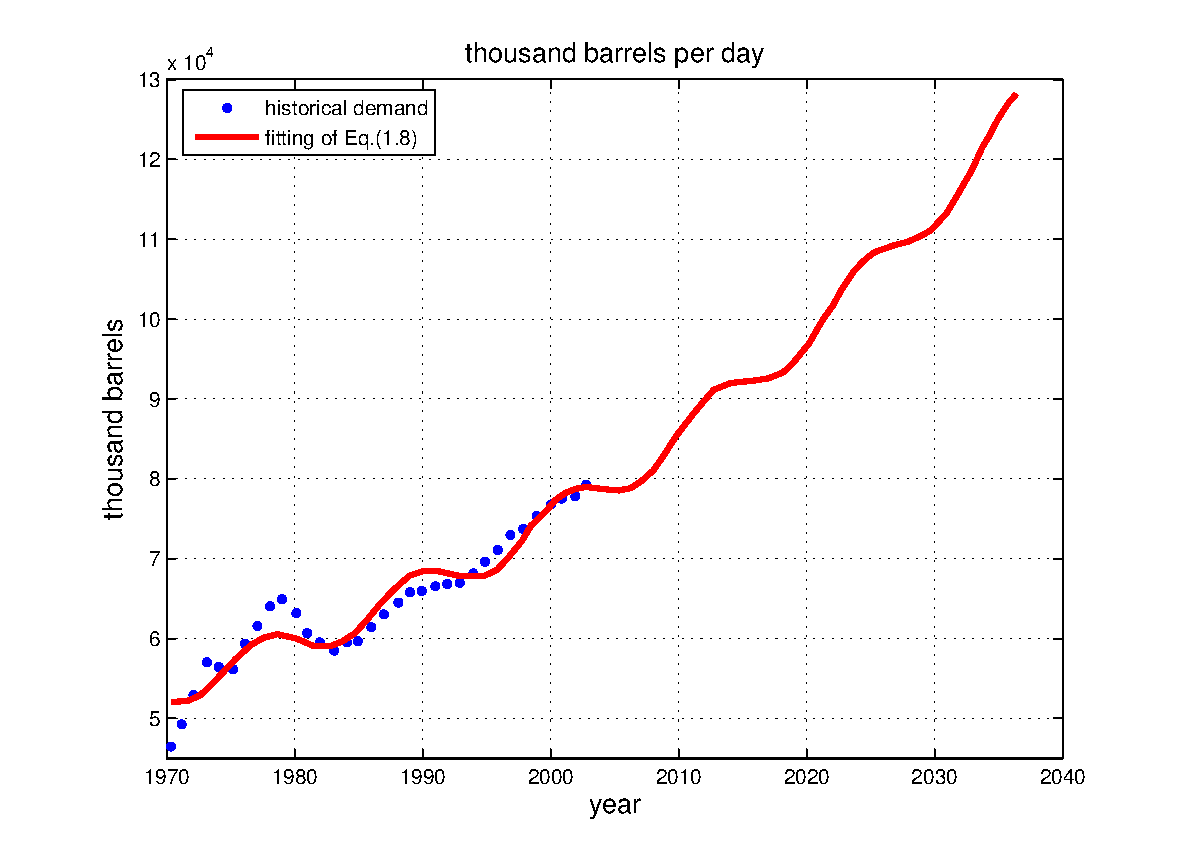
\includegraphics[width=0.7\textwidth]{fig01.eps}
\caption{The fitting curve by Eq.(2)}
\end{figure}



Noticing that with the passing of time, the third term
($a_5\exp(a_6t)$) on the right side of Eq.(2) will play a more
important role and the second term$(a_{2}\cos(a_{3}t+a_{4}))$ can
be neglected, thus for the sake of convenience, we reduce Eq.(2)
to:


\begin{equation}
D(t)=a_{1}+a_{5}\exp(a_{6}t)
\end{equation}

Hence we choose exponential fitting to predict future demand, and
for the purpose of comparison, we also choose linear fitting and a
invariable demand case in which future demand is assumed the same
as that of 2003. The data for fitting is world-wide oil demand
$D(i)(i=1970,\ldots,2003)$ in Table 1 , and the fitting results
are given as follows:

Exponential fitting:\[
D(t)=365*(29820+2.265*10^{-15}*\exp(0.02223*t))  (t\geq 2004)
\]

Linear fitting:\[  D(t)=365*(771.2*t+(-1.467e+006))   (t\geq 2004)
\]

The predicted demand is shown in Figure 2. (For convenience,
annual demand is in the form of average daily demand.)

\begin{figure}[!htb] \centering
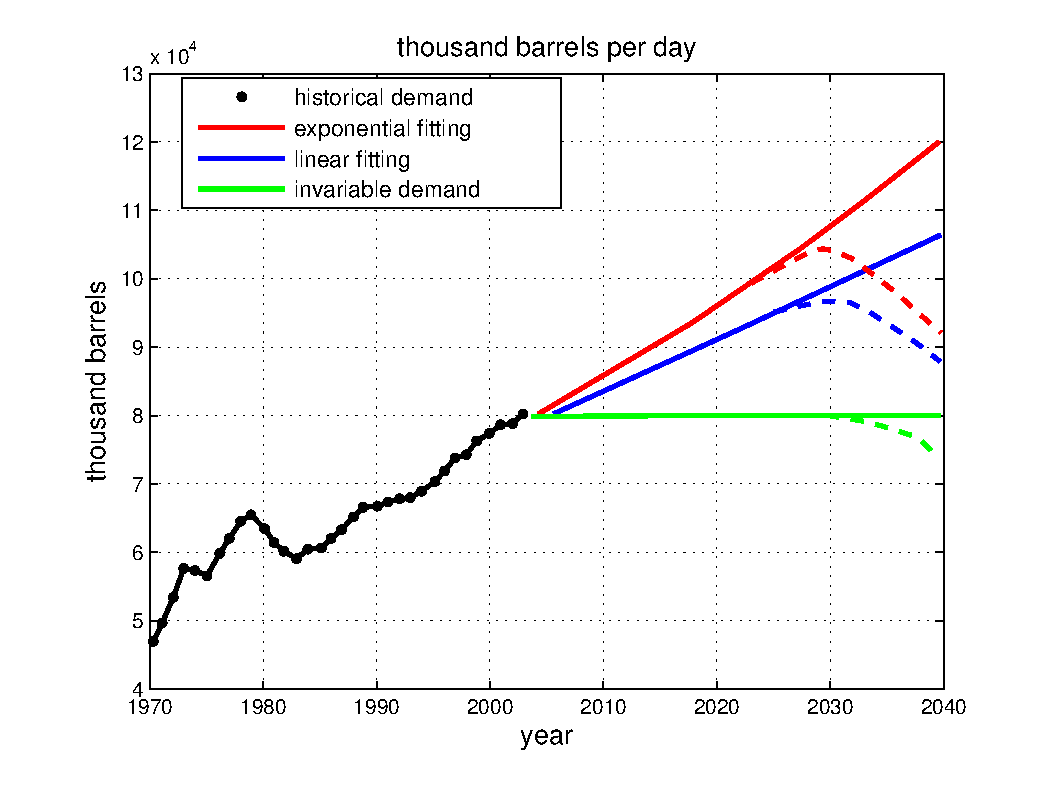
\includegraphics[width=0.7\textwidth]{fig02.eps}
\caption{Estimation of future oil demand}
\end{figure}

\textit{Remark: With the increase of oil demand, its price will
accordingly rise. As is shown by the broken lines in figure 2,
this will lead to the decline of oil demand, and we will discuss
this phenomenon in detail later.}


\subsection{Sensitivity Analysis:}

Based on the above assumption,$U(t)$ is the undiscovered oil on
earth at year $t$, so it is difficult to get a precise value. What
we can acquire is merely an estimation, which may contain a
certain degree of deviation. We now investigate whether the
deviation will bring about a serious distortion on the
determination on $n$.

We give $U(t)(t=1997)$ a fluctuation of $\pm10\%$, and study the
corresponding change of $n$. The conclusion is shown in Table 2.

From table 2, we can learn that the fluctuation of $U(t)$ does not
have a strong influence on the estimated year of oil's exhaustion.

\begin{table}
\centering \caption{the relationship between the fluctuation of
$U(t)$ and the year of oil exhaustion}
\begin{tabular}{|l|l|lll|lll|lll|}
\hlinewd{1pt}
\multicolumn{2}{|c|}{The year of oil exhaustion($n$)} & \multicolumn{9}{c|}{Fluctuation of $u(t)$(t=2000)} \\
\hlinewd{1pt}
\multicolumn{1}{|c|}{} & \multicolumn{1}{c|}{Exponential} & \multicolumn{1}{c}{} & \multicolumn{1}{c}{-10\%} & \multicolumn{1}{c|}{} & \multicolumn{1}{c}{} & \multicolumn{1}{c}{0\%} & \multicolumn{1}{c|}{} & \multicolumn{1}{c}{} & \multicolumn{1}{c}{+10\%} & \multicolumn{1}{c|}{} \\
\cline{2-11}
\multicolumn{1}{|c|}{The way of} & \multicolumn{1}{c|}{Linear} & \multicolumn{1}{c}{} & 2032 &  & \multicolumn{1}{c}{} & \multicolumn{1}{c}{2032} & \multicolumn{1}{c|}{} & \multicolumn{1}{c}{} & \multicolumn{1}{c}{2032} & \multicolumn{1}{c|}{} \\
\cline{2-11}
\multicolumn{1}{|c|}{fitting} & \multicolumn{1}{c|}{Invariable} & \multicolumn{1}{c}{} & \multicolumn{1}{c}{2033} & \multicolumn{1}{c|}{} & \multicolumn{1}{c}{} & \multicolumn{1}{c}{2033} & \multicolumn{1}{c|}{} & \multicolumn{1}{c}{} & \multicolumn{1}{c}{2034} & \multicolumn{1}{c|}{} \\
\cline{2-11}
\multicolumn{1}{|c|}{} & \multicolumn{1}{c|}{demand case} & \multicolumn{1}{c}{} & \multicolumn{1}{c}{2036} & \multicolumn{1}{c|}{} & \multicolumn{1}{c}{} & \multicolumn{1}{c}{2037} & \multicolumn{1}{c|}{} & \multicolumn{1}{c}{} & \multicolumn{1}{c}{2037} & \multicolumn{1}{c|}{} \\
\hlinewd{1pt}
\end{tabular}
\end{table}


\section{Task 2  The Influence of Economic, Demographic, Political and Environmental Factors on the Oil}

\subsection{Assumptions}
\begin{enumerate}
\item We assume that the annual demand of oil could reflect the annual consumption of oil.

\item When we consider the effect of one factor, the other factors
are neglected, in other words, we do not take the interaction of
arbitrary two different factors into account.

\item When considering the future consumption of oil, we ignore the
intrinsic fluctuation, because its influence is really small. That
means we only consider the tendency of the future tendency.
\end{enumerate}


In task 1, we've assumed that oil demand is in an exponential
form, but in reality, many factors such as economy, population,
politics and environment, will influence oil consumption. Thus, in
the following discussion, we modify the model provided in Task 1
to include the above-mentioned factors and thereby make our
results more approximate to the reality.


\subsection{The Influence of Economic Factors}

We use GDP as the measure of economy. First we investigate the
relationship between demand and supply. Based on the data of
worldwide oil demand and supply between 1970 and 2003, we perform
a correlation analysis between oil demand and oil supply, and get
the correlation coefficient $r= 0.9911$. Therefore, we justifiably
deem that demand is almost linearly dependent on supply. So when
we consider the influence of oil on demand, caused by economic, we
take the demand as a dependent variable. And the data we obtain
about the recent world total GDP is shown in Table 3, while the
data about the total world oil consumption in recent years is
shown in Table 4.

\begin{table}[!htb]
\centering \caption{Recent World Total GDP(\$ 108),1995-2003}
\begin{tabular}{lllllllll}
\hlinewd{1pt}
\multicolumn{1}{c}{1995} & \multicolumn{1}{c}{1996} & \multicolumn{1}{c}{1997} & \multicolumn{1}{c}{1998} & \multicolumn{1}{c}{1999} & \multicolumn{1}{c}{2000} & \multicolumn{1}{c}{2001} & \multicolumn{1}{c}{2002} & \multicolumn{1}{c}{2003} \\
\hline
\multicolumn{1}{c}{27.134} & \multicolumn{1}{c}{28.247} & \multicolumn{1}{c}{29.433} & \multicolumn{1}{c}{30.257} & \multicolumn{1}{c}{31.377} & \multicolumn{1}{c}{32.85} & \multicolumn{1}{c}{33.64} & \multicolumn{1}{c}{34.6487} & \multicolumn{1}{c}{36} \\
\hlinewd{1pt}
\end{tabular}
\end{table}



\begin{table}[!htb]
\centering \caption{Recent Total World Oil Consumption($10^3$
thousands of barrels/day),1995-2003}
\begin{tabular}{lllllllll}
\hlinewd{1pt}
\multicolumn{1}{c}{1995} & \multicolumn{1}{c}{1996} & \multicolumn{1}{c}{1997} & \multicolumn{1}{c}{1998} & \multicolumn{1}{c}{1999} & \multicolumn{1}{c}{2000} & \multicolumn{1}{c}{2001} & \multicolumn{1}{c}{2002} & \multicolumn{1}{c}{2003} \\
\hline
\multicolumn{1}{c}{69955} & \multicolumn{1}{c}{71522} & \multicolumn{1}{c}{73292} & \multicolumn{1}{c}{73932} & \multicolumn{1}{c}{75826} & \multicolumn{1}{c}{76954} & \multicolumn{1}{c}{78105} & \multicolumn{1}{c}{78439} & \multicolumn{1}{c}{79813} \\
\hlinewd{1pt}
\end{tabular}
\end{table}

We know from the table that the GDP value and the worldwide oil
consumption both increase as time elapses. Hence we make a
correlation analysis for these two lists of data, and the
correlation coefficient turns out to be 0.9930. That is to say,
the GDP value and oil consumption are of strong positive linear
dependence.

In order to find out the intrinsic relationship between them, we
make a linear regression for these data. The regression equation
is given as follows:


\begin{equation}
y=1183\times x+38140
\end{equation}


\newenvironment{vardesc}[1]{%
\settowidth{\parindent}{#1\ } \makebox[0pt][r]{#1\ }}{}

\begin{vardesc}{Where}$x$: global GDP value

$y$: worldwide oil consumption
\end{vardesc}

And \textit{R-square}.(square of regression coefficient) is
0.9861. And the further statistical significance test shows that
there indeed exists a linear dependence between the global GDP
value and worldwide oil consumption.

Next, using Eq.(4), we can predict the cumulative oil demand as
the global GDP grows at the rate of 10\%, 5\%, 3\%, 1\%
respectively. For the convenience, we take the year 2001 as the
starting point, and we get that the total remaining oil on earth
at that time is $1.1178\times 10^{+12}$(barrels). And then we
calculate the time of the oil exhaustion under different cases of
economic growth. Oil depletion time is shown in the following
figure:

\begin{figure}[!htb] \centering
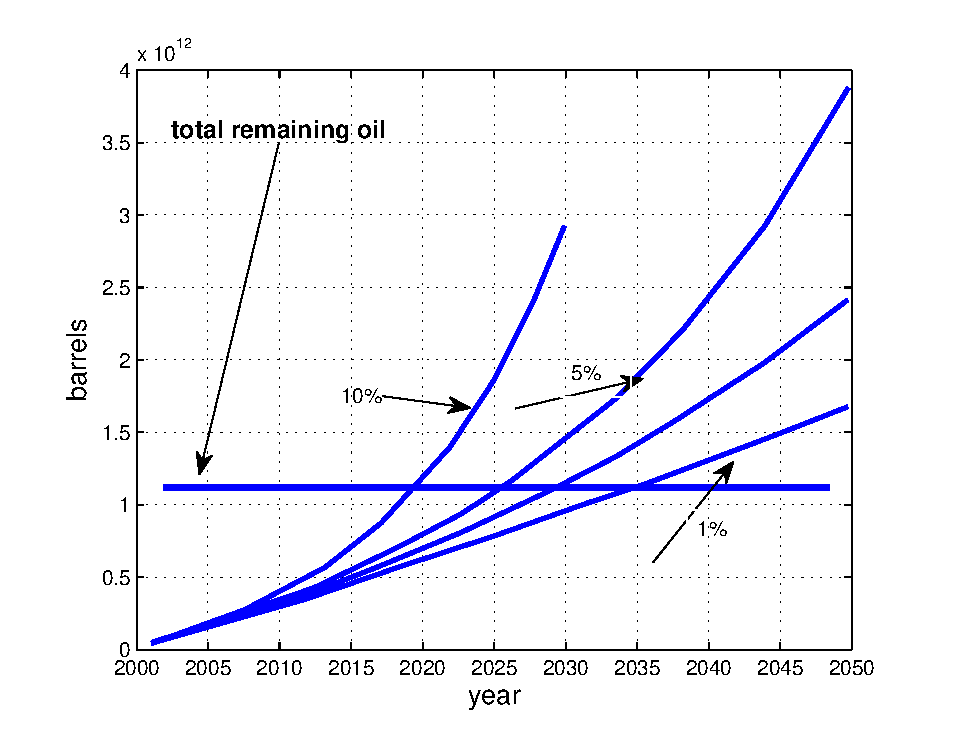
\includegraphics[width=0.7\textwidth]{fig03.eps}
\caption{the curves of cumulative consumption under different
rates of GDP growth}
\end{figure}

The horizontal line denotes the total remaining oil at year 2001.
The x-axis coordinates of the intersection points of the
horizontal line and the curves denote oil exhaustion time at the
GDP growth rate of 10\%, 5\%, 3\%, 1\% , respectively.


We find that the faster the GDP growth rate is, the larger the oil
consumption will be, making the advent of the exhaustion time to
come sooner. When the GDP growth rate is 10\%, oil will be
depleted at 2020; when the GDP growth rate is 5\%, oil will be
used up at 2026; When the GDP growth rate is 3\%, oil will be used
out at 2029,and finally, When the GDP growth rate is 1\%, oil will
be used out at 2035.


As for a specific nation, its GDP growth rate can be controlled
through some economic approaches, so as to delay the advent of oil
exhaustion.



\subsection{The Demographic Influence on Oil Consumption}

First, we resort to \emph{\textbf{Logistic}} model to predict the
change of world population in years to come. The model is as
follows:


\begin{equation}
x(t)=\frac{k}{1+(\frac{k}{x_{0}}-1)e^{-(t-t_{0})r}}
\end{equation}

\newenvironment{vardesc}[1]{%
\settowidth{\parindent}{#1\ } \makebox[0pt][r]{#1\ }}{}

\begin{vardesc}{Where}$t$: denotes time;

$t_{0}$: denotes initial time;

$x_{0}$: denotes the population at initial time;

$k$: is the environment capacity, namely the maximum number of
population the earth can accommodate;

$r$: is the intrinsic growth rate of population.

\end{vardesc}

We use the data of the population in recent decades to fit the
above equation, and get the formula of the change of population
with time:

\begin{equation}
x(t)=\frac{100}{1+(\frac{100}{44.585}-1)e^{-0.0327\times
(t-1980)}}
\end{equation}

Now, using Eq. (6) we can the prediction of future population,
which is shown in the following table:

\begin{table}[!htb]
\centering \caption{The population estimated by the
\emph{\textbf{Logistic model}}(0.1billion)}
\begin{tabular}{lllllllll}
\hlinewd{1pt}
\multicolumn{1}{c}{1980} & \multicolumn{1}{c}{1990} & \multicolumn{1}{c}{2000} & \multicolumn{1}{c}{2010} & \multicolumn{1}{c}{2020} & \multicolumn{1}{c}{2030} & \multicolumn{1}{c}{3040} & \multicolumn{1}{c}{2050} & \multicolumn{1}{c}{2060} \\
\hline
\multicolumn{1}{c}{44.585} & \multicolumn{1}{c}{52.736} & \multicolumn{1}{c}{60.744} & \multicolumn{1}{c}{68.212} & \multicolumn{1}{c}{74.849} & \multicolumn{1}{c}{80.495} & \multicolumn{1}{c}{85.126} & \multicolumn{1}{c}{88.811} & \multicolumn{1}{c}{91.560} \\
\hlinewd{1pt}
\end{tabular}
\end{table}

Similarly, we try to obtain the relationship between oil
consumption and total population as we do in the section of
studying GDP's influence. The correlation coefficient is 0.9877.
Obviously, there exists a strong positive linear dependence
between oil consumption and total population. Theoretically, the
larger the population is, the greater the oil demand will be,
which coincides with the above result.

Naturally, we make a linear regression for oil demand and
population, and get the relationship between them as follows:

\begin{equation}
y=1443\times x-11170
\end{equation}



\newenvironment{vardesc}[1]{%
\settowidth{\parindent}{#1\ } \makebox[0pt][r]{#1\ }}{}

\begin{vardesc}{Where}$y$: oil consumption;.

$x$: total population.
\end{vardesc}


From (6) we can get the future population, and from (7) we may
obtain oil demand in the future. Hence, the time of oil exhaustion
can be estimated under such a growth of population.

\begin{figure}[!htb] \centering
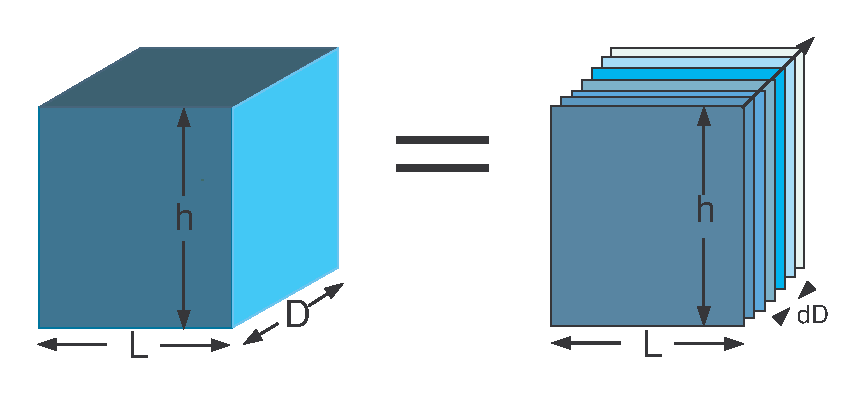
\includegraphics[width=0.7\textwidth]{fig04.eps}
\caption{the curve of cumulative oil consumption with the growth
of population}
\end{figure}

From the above figure we can clearly see that oil will be in the
state of exhaustion if population increases in the way of (6). And
the intersection point of the horizontal line and the curve is the
corresponding exhaustion time under a specific growth rate of
population, which is not difficult to estimate.


\subsection{The Political Influence on Oil Consumption}

Here, we mainly discuss the influences caused by wars.


In Task 1, we have fitted the function of demand dependent on time
as follows:

\[
y(t)=7.95\times 10^{-6}\times e^{0.01149t}
\]

from which we can estimate the oil demand at any given time. Let
rate denote the growth rate of oil consumption, thus


\[
rate=\frac{y(t+1)}{y(t)}-1=\frac{7.95\times 10^{-6}\times
e^{0.01149(t+1)}}{7.95\times 10^{-6}\times
e^{0.01149t}}-1=e^{0.01149}-1 =1.56\%
\]

From the above equation, we find that the annual growth rate of
oil consumption remains at the same level of 1.56\% if oil
consumption increases in an exponential form, and we call it
\emph{\textbf{average growth rate}}.

Now, we investigate the growth rate of oil consumption during the
past decades, and the results are shown in the figure below.

\begin{figure}[!htb] \centering
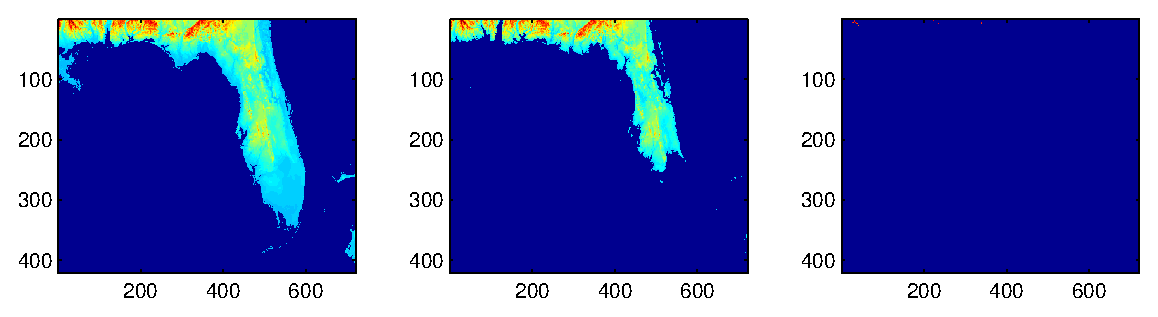
\includegraphics[width=0.7\textwidth]{fig05.eps}
\caption{the curve of oil consumption growth rate and mean growth
rate}
\end{figure}

From the figure above, we can obviously see that the growth rate
declines sharply in the year 1974 1980 and 1990, which coincides
with the outbreak of the fourth Middle East War (1973), the
Iran-Iraq War (1980) and the Gulf War (1990). And these three wars
all broke out in the Middle East, which is the center of oil
production. So the wars strongly impacted the oil price, and
consequently impacted the oil demand.


Define
\begin{equation}
\Delta rate=rate(t)-\overline{rate}
\end{equation}

\newenvironment{vardesc}[1]{%
\settowidth{\parindent}{#1\ } \makebox[0pt][r]{#1\ }}{}

\begin{vardesc}{Where}$rate(t)$: the growth rate of oil consumption at year $t$

$\overline{rate}$: the average growth rate of oil consumption
\end{vardesc}





So $\Delta rate$ indicates the deviation of oil assumption off its
mean level. We calculate the $\Delta rate$ in year 1974, 1980 and
1990, respectively, and the three numbers may reflect the affects
on oil demand caused by these three wars, respectively. The
results are in the table below.

\begin{table}[!htb]
\centering \caption{$\Delta$ rate in year 1974,1980 and 1990}
\begin{tabular}{lll}
\hlinewd{1pt}
\multicolumn{1}{c}{1974} & \multicolumn{1}{c}{1980} & \multicolumn{1}{c}{1990} \\
\hline
\multicolumn{1}{c}{-0.02533} & \multicolumn{1}{c}{-0.048} & \multicolumn{1}{c}{-0.0103} \\
\hlinewd{1pt}
\end{tabular}
\end{table}

We reach the conclusion that wars will make the growth rate of oil
consumption well bellow its average level.

As for other political influences, we can use the similar method,
and the key is to choose the crucial factor to analysis.

\subsection{The Environmental Influence on Oil Consumption}

The use of oil inevitably leads to environment pollution. To
protect the environment against excessive pollution, the
government would adopt certain measures to limit the use of oil.
So the environmental factors will also influence the oil demand.


We take the discharge amount of carbon dioxide generated by oil
consumption as the scale to measure the environment pollution, and
study the relation between the discharge amount of carbon dioxide
and oil consumption. The data of discharge amount of carbon
dioxide is shown in the table below.

\begin{table}[!htb]
\centering \caption{World Carbon Dioxide Emissions From the
Consumption of Oil (million metric tons of carbon dioxide)}
\begin{tabular}{lllllllll}
\hlinewd{1pt}
\multicolumn{1}{c}{1993} & \multicolumn{1}{c}{1994} & \multicolumn{1}{c}{1995} & \multicolumn{1}{c}{1996} & \multicolumn{1}{c}{1997} & \multicolumn{1}{c}{1998} & \multicolumn{1}{c}{1999} & \multicolumn{1}{c}{2000} & \multicolumn{1}{c}{2001} \\
\hline
\multicolumn{1}{r}{9220} & \multicolumn{1}{r}{9284} & \multicolumn{1}{r}{9388} & \multicolumn{1}{r}{9586} & \multicolumn{1}{r}{9691} & \multicolumn{1}{r}{9766} & \multicolumn{1}{r}{9939} & \multicolumn{1}{r}{10138} & \multicolumn{1}{r}{10292} \\
\hlinewd{1pt}
\end{tabular}
\end{table}

First, we also make a correlation analysis for the discharge
amount of carbon dioxide and oil consumption, and the correlation
coefficient is 0.9937. That is to say, the two variables are of
strong positive linear dependence. Then we make a linear
regression, and get the relationship between carbon dioxide
emission and oil consumption as follows:


\begin{equation}
y=10.09\times x-25320
\end{equation}


\newenvironment{vardesc}[1]{%
\settowidth{\parindent}{#1\ } \makebox[0pt][r]{#1\ }}{}

\begin{vardesc}{Where}$y$: oil consumption;

$x$: discharge amount of carbon dioxide caused by oil consumption.
\end{vardesc}



From Eq $(9)$ we can work out the oil consumption at a controlled
annual $\textrm{CO}_{2}$ emission growth rate. We simulate the
future oil consumption under different annual $\textrm{CO}_{2}$
emission growth rate of 1\%, 3\%\ldots The corresponding oil
exhaustion time is shown in the figure below.

\begin{figure}[!htb] \centering
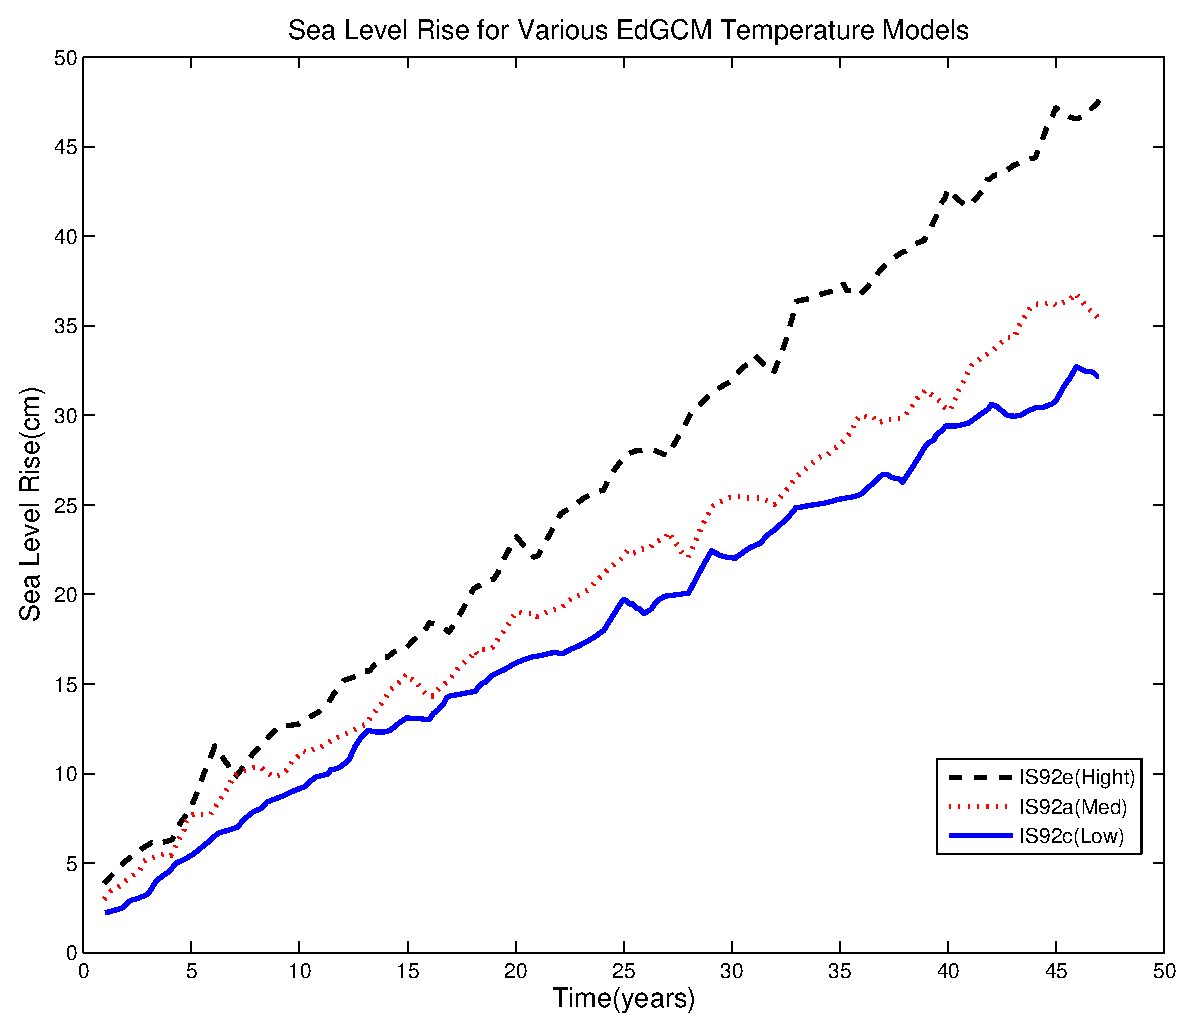
\includegraphics[width=0.7\textwidth]{fig06.eps}
\caption{the curve of cumulative oil consumption under different
annual $\textrm{CO}_2$ emission growth rates}
\end{figure}


Based on the analysis above, if we want to keep the annual
$\textrm{CO}_{2}$ emission growth rate at a given level, we can
give the corresponding annual oil consumption, and then fulfill
the purpose of protecting the environment.

\subsection{Limitations}

The above models are based on the assumption that all the other
factors are invariable when modeling for a specific factor. But
this cannot be true in reality, because one factor may be
interacted with others. Thus, the interactions should be taken
into account in further study.


\section{Task 3 The Sustainable Use of Oil}

In order to prevent the excessive consumption of nonrenewable
resource from rapid depletion, and to take into account of our
offspring's interests, we must develop a policy to control the
consumption of nonrenewable resource to give a rational
consumption allocation between generations.


\subsection{Assumptions}

\begin{enumerate}
\item We assume that annual demand of oil can truly reflect oil consumption.

\item Oil consumption in year $t$ can not be far less than that in
year $t-1$.

\item The sustainable use of oil means that we must
take the needs of our offspring into account. That is to say, we
should provide a rational consumption allocation between
generations.

\item We assume that one generation consists of $n$ years.

\end{enumerate}

\subsection{The Criterion of Rational Consumption Allocation of Oil Between Generations.}

Based on Task 1, we know that $U(t)+R(t)$ denotes the total
remaining oil on earth at year $t$, and obviously, it holds that:


\begin{equation}
U(t)+R(t)=m_{1}+m_{2}
\end{equation}

\newenvironment{vardesc}[1]{%
\settowidth{\parindent}{#1\ } \makebox[0pt][r]{#1\ }}{}

\begin{vardesc}{Where}$m_{1}$: the amount of oil for contemporary man;

$m_{2}$: the amount of oil left for offspring.
\end{vardesc}

In order to give a rational allocation, we define:


\begin{equation}
\eta=\frac{m_{2}}{m_{1}}\times 100\%       (0\leq \eta \leq
\infty)
\end{equation}

$\eta$ is called \textbf{the degree of rational consumption
allocation of oil.}


A large value of $\eta$ indicates a high degree of rational
consumption allocation, and vice versa. But if the value of $\eta$
is too high, the amount of oil for contemporary human beings is
too small to meet the needs. So we may give an alert analysis and
management by choosing a suitable critical value of $\eta$, say
$\eta'$. Having known the value of $\eta'$, we can obtain the
optimal allocation in the n years of one generation.


\subsection{Modeling the Rational Consumption Allocation}

We hope that future oil demand will not undergo a sharp decline,
and expect oil to be allocated among generations fairly.
Meanwhile, we wish that the resource is utilized in the most
efficient way.


As is assumed, one generation consists of n years, and now we
model at the interval of $n$ years, i.e. one generation. Based on
the assumptions, we can construct the following optimization
model:

\[
\max\sum^{n}_{i=1}c_{i}\times d_{i}
\]

\begin{equation}
s.t.=\left\{\begin{array}{ll}
\frac{r}{\sum_{i=1}^nd_i}\geq\eta'\\
d_i\geq a\times d_{i-1},i=1,2,\cdots,n\\
d_i\geq 0,i=1,2,\cdots,n \end{array}\right\end{equation}

\newenvironment{vardesc}[1]{%
\settowidth{\parindent}{#1\ } \makebox[0pt][r]{#1\ }}{}

\begin{vardesc}{Where}$c_{i}$: the utilization rate of oil at year $i$;

$\eta'$: the degree of rational consumption allocation of oil
between generations.

$d_{i}$: oil consumption at year $i$, and $d_{0}$ indicates oil
consumption at initial time.

$r$: the total remaining oil in the first year of one generation.

$\alpha$: a given percentage such that the oil consumption at a
given year must not be less than $\alpha$ times the consumption in
the previous year. And $\alpha$ is close to 1.


\end{vardesc}

The objective here is to obtain the maximum total utilization rate
of oil in n years. The first constraint condition assures a high
rate of rational oil allocation between generations, while
$d_{i}\geq \alpha\times d_{i-1},i=1,2,\cdots,n$ makes sure that
the oil consumption at year $i$ is not less than $\alpha$ times
the consumption at year $i-1(i=1,\ldots,n)$. The purpose is to
guarantee a smooth oil demand change.


When $\eta',c_{i},r,\alpha$ is given, we can obtain the optimal
consumption allocation of oil between $n$ years by solving the
linear programming (12). As for the estimation of $c_{i}$ here, we
believe that the utilization rate should increase as time passes
by, but is always smaller than 1, nevertheless. Thus,$c_{i}$ can
be regarded as in the following form:


\begin{equation}
c_{i}=1-a_{1}e^{a_{2}t}
\end{equation}


where $a_{1}$ and $a_{2}$ are constants and can be determined by
fitting historical data.

The result we get here may not increase in an exponential way.
After determining the annual consumption, we can adjust it to
include the factors such as economy, demography, politics and so
on, until it is optimal.


Next, we give an illustration to show the consumption under
optimal allocation after year 2004. For instance, we set
$\alpha=1$, $\eta'=1.67$, $r=1.0\times 10^{12}$ and year 2004 to
be the base time, i.e.$d_{0}$ is the oil consumption at 2004. Thus
we can give the prediction of the oil consumption after 2005,
which is shown in the following figure.

\begin{figure}[!htb] \centering
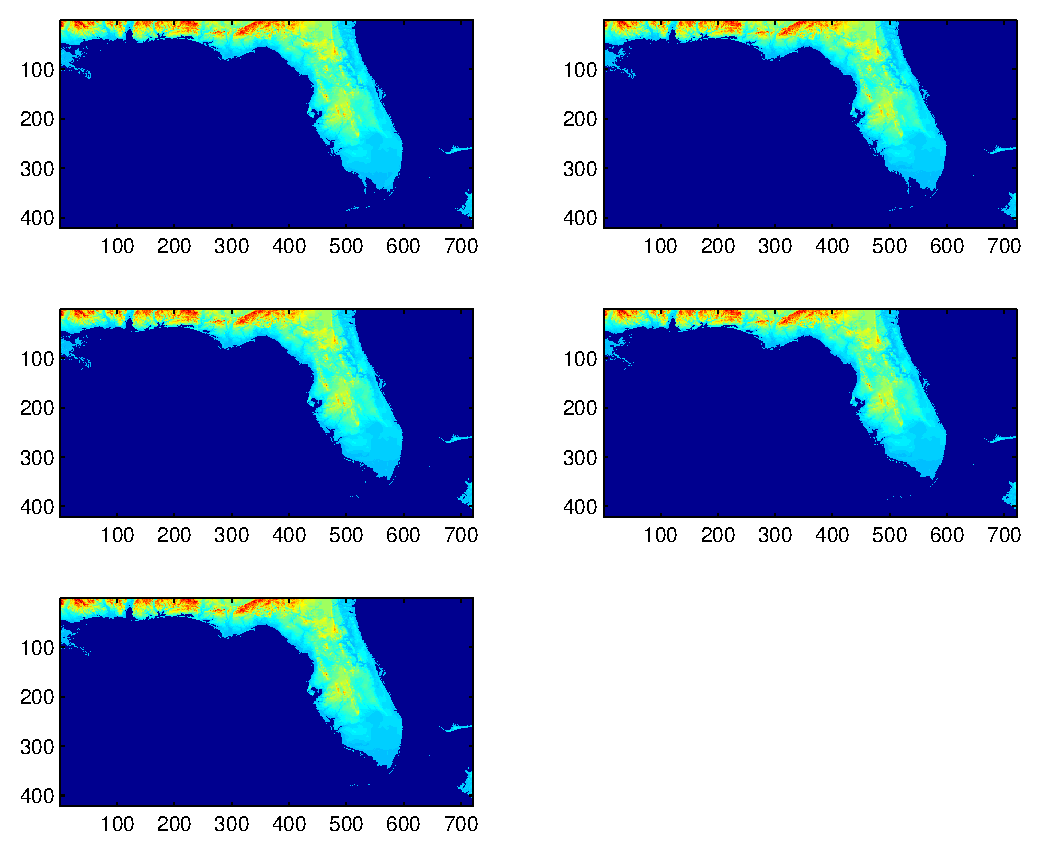
\includegraphics[width=0.7\textwidth]{fig07.eps}
\caption{Oil Consumption Under Optimal Allocation}
\end{figure}

From the above figure, we can find that annual oil consumption
under optimal allocation is far less than that in an exponential
way. That is to say, the optimal consumption varies smoothly. But
in the late phase of the prediction, consumption fluctuates
sharply. This is due to the reason that we may have chosen an
inappropriate $\eta'$-value. However, the choosing of
$\eta'$-value is rather difficult because it should incorporate
many factors such as population, price, specific economic
environment, etc. Fortunately, the data at the prophase can
clearly reflect the trend of oil consumption.

\subsection{The Policy}
To guarantee a sufficient amount of oil for our offspring to
sustain their development, we must keep a rational allocation of
oil. This can be done through the following measurements:

\begin{enumerate}

\item We may levy a relatively heavy tax on oil compared with other resources.

\item We should encourage the development of alternatives for oil.

\end{enumerate}

'Security' Policy for Oil} We believe that the problem of oil
security arises mainly due to the different utilization rates
among countries. For example, if a country with low oil
utilization rate is assigned a redundancy of oil, whereas a
country with high utilization rate is assigned an insufficient
amount of oil, this phenomenon will lead to a great waste. Based
on this idea, we can establish one model to find out the optimal
distribution of oil among the countries with different utilization
rates.

\subsection{Assumptions:}
\begin{enumerate}
\item The utilization rates among countries are different.

\item The low utilization rate is the primary source to result
in the misuse and waste of oil.

\item The annual oil consumption of the whole world is according
to optimal oil allocation model in Task 3

\item We do not take the trade barrier into account, and assume
that reallocation of oil between countries is feasible.
\end{enumerate}


\subsection{Modeling:}
Suppose there are $n$ main oil-consuming countries in the world.
Given the year $t$, we can establish the linear programming as
follows:

\[
\max\sum^{n}_{i=1}l_{i}(t) \times x_{i}(t)
\]

\begin{equation}
s.t.\left\{\begin{array}{ll}\sum^{n}_{i=1}x_{i}(t)=d(t)}}\\
x_i(t)\geq\alpha_i(t)\times x_i(t-1),i=1,2,\cdots,n\\
x_i(t)\geq 0,i=1,2,\cdots,n \end{array}\right
\end{equation}


\begin{vardesc}{Where}$l_{i}(t)$ : the oil utilization rate of country $i$ at year
$t$;

$x_{i}(t)$: the oil consumption of country $i$ at year $t$;


$d(t)$: the world-wide oil consumption allocation at year $t$,
which can be obtained using the model in Task 3.

$\alpha_{i}(t)$: the minimum ratio of $x_{i}(t)$ to
$x_{i}(t-1)$.in percentage.
\end{vardesc}



Remark: $\alpha_{i}(t)$, as a parameter, is close to 1, and it
needs to be evaluated according to the different situations and
the rationality of oil consumption of countries.

The first constraint condition means the sum of oil consumption of
different countries at year $t$ should equal total oil consumption
at year $t$ under optimal oil allocation.

The constraint condition $x_{i}(t) \geq \alpha_{i}(t) \times
x_{i}(t-1),i=1,2...,n$ means the oil consumption of country $i$ at
year $t$ is not less than a certain degree of the previous year's
consumption. This degree is different among countries. From this
model, we can see that the country with higher oil utilization
rate has relative privilege to get the oil supply. The optimal
solution of the linear programming represents the optimal oil
distribution among countries at year $t$. Thus, we can meet the
needs of every country with the minimal waste of oil.

\subsection{Limitations of the model}
The model we have designed above is for the sake of the interest
of the entire world, but in reality, countries would more likely
consider their own interests, leading to the result of tight trade
barriers among countries, and consequently making it impossible to
get the optimal distribution.

\subsection{Conclusion}
For a country with large oil demand but low utilization rate, we
should fulfill its consume level while cut down the extra oil
demand, while for a country with small oil demand but high
utilization rate, we should meet its demand to the maximum extent,
in order to prevent oil waste.

\subsection{The Policy}
To assure a good utilization of oil, and reduce unnecessary waste,
we give the following measurements:

\begin{enumerate}

\item We may levy a relatively heavy tax on oil to countries with
low utilization rate.

\item We can set a limit on the annual oil consumption for countries with low utilization rate
\end{enumerate}


\section{Task 5 Oil Exploitation vs. Natural Disasters}

Oil exploitation is a tough task because the nature is very
vulnerable. And if our activities go against the intrinsic laws of
nature, we will be punished by it. Oilfield occupies a large range
of area, destroys the vegetation in the vicinity, changes the
components of the soil, and deteriorates the environment near by,
and hence the animals will lose their habitat. With the
exploitation of the field, it will influence the groundwater and
cause desertification. An obvious instance is oil spill, which
often leads to the pollution of nearby water area, and further
destroys the entire water area eco-system.

Next, we mainly consider the effects of oil exploitation on
natural disasters. We hope that the susceptibilities to disasters
to be as low as possible while the demand for oil is satisfied.


\subsection{Assumptions}
\begin{enumerate}
\item The amount of oil exploited entirely turns into consumption.

\item The total amount of oil exploited can meet the need of
economic development.
\end{enumerate}

\subsection{Modeling the short-term effects}

We mainly consider the short-term effects, and assume that the
total number of oilfields on the earth is $n$. According to the
first assumption, oil exploitation is at the same level of oil
consumption. In order to satisfy the sustainable development of
the economy, we must try to keep the total output of all oilfields
to be the same as the world-wide oil consumption under optimal
allocation in Task 3. Thus, we have the following equation:

\begin{equation}
\sum^{n}_{i=1}x_{i}(t)=d(t)
\end{equation}


\begin{vardesc}{Where}$x_{i}(t)$: the output of the ith oilfield at year $t$;

$d(t)$: the world wide oil consumption under optimal oil
allocation in Task 3.
\end{vardesc}

For a specific oilfield $i$,we believe that its susceptibility to
disasters has something to do with its output at a given year and
the ratio of its cumulative output to its initial oil reserve.

Naturally, the more the oil is exploited, the greater the
likelihood of disasters will be. We believe that they are of
linear independence. And of course, a new oilfield and an old one
will have different effects on the environment. This difference is
shown by the ratio of the cumulative output to the initial oil
reserve. Here we introduce a penalty function
$e^{-\alpha(1-\lambda_{i}(t))}$,and get the following equation:

\begin{equation}
p_{i}(t)=k_{i}\times x_{i}(t)\times e^{-\alpha(1-\lambda_{i}(t))},
\end{equation}

\begin{vardesc}{Where}$k_{i}$: proportion coefficient, which is determined by the
position and exploitation method of the oilfield. Here, a small
value of $k_{i}$ represents a prior position and an advanced
exploitation method.

$p_{i}$: the susceptibility to disasters.

$\lambda_{i}(t)$: the ith oilfield's ratio of its cumulative
output until year $t$ to its initial oil reserve.
\end{vardesc}

We hope to minimize the total susceptibilities of different
oilfields under the condition that the worldwide oil demands can
be satisfied. That is:

\[
\min\sum^{n}_{i=1}p_{i}(t)
\]
\[
s.t.\sum^{n}_{i=1}x_{i}(t)=d(t)
\]

The solution to this optimization problem generates the outputs of
every oilfield that can assure the least possibility to disasters.
Obviously, we find out those oilfields with small value of $k_{i}$
will have larger outputs and vice versa.

We also increase the value of $n$ tentatively, i.e. to increase
the number of oilfields, and find that the total susceptibilities
will decrease. This is mainly due to the fact that during the
prophase of exploitation,$\exp^{-\alpha(1-\lambda_{i}(t))}$ plays
an important role, leading to the exploitation of new oilfields,
and this will decrease the likelihood of disasters.


\subsection{The Policy}

Our policy is to increase the output of old oilfields with small
$k_{i}$-value (those with a prior position and a priority of
exploitation), and reduce the output of those with large
$k_{i}$-value (those with an inferior position and a backward
exploitation method). Also, if possible, we should exploit as many
new oilfields as possible and decrease the exploitation of old
oilfields, so as to control the susceptibilities to disaster.

\subsection{Long-term Effects} As for the long-term effects, for a
given oilfield, the average annual output should be minimal. So it
allows us to carry out an intensive exploitation in one year and
then a mild one in another. By doing so, there is no necessity for
us to increase the number of new oilfields in a short time, and
the benefit is that it allows us to have enough time to search for
and construct new oil fields.


\section{Task 6 The Development of The Alternatives for Oil}

With the development of human, oil is being used ceaselessly. And
we have estimated that if oil consumption increases in an
exponential way, it will be used out in about thirty years. Even
if we control the use of it, the time can only be prolonged by
four to five years. So, at present stage, we urgently need an
alternative for oil. For the sake of sustainable development, we
must gradually accelerate the consumption of oil's alternative at
the anaphase of the depletion of oil. The question is how should
we apply the alternative in order to keep the economy stable
during the transition period.

\subsection{Assumptions}

\begin{enumerate}
\item We only consider one kind of alternative.
\item Oil and its alternative have precisely the same function as energy resource .
\item The criterion of the measurement of oil and its alternative is their contributions to GDP.
\item We assume that the quantity of oil to produce unit of energy will not change as time elapses.
\end{enumerate}

\subsection{Analysis}

We assume that the cost for oil to produce unit energy is $c_{1}$,
and that of its alternative is $c_{2}$ m such that $c_{1}\leq
c_{2}$. This is on the basis the fact that the cost for oil to
produce unit energy is lowest compared with any other resources
(See [5]). Because of this, the consumption of oil is far greater
than those of its alternative.

But we must realize the fact that the total amount of remaining
oil on the earth is declining, so the price of oil will
correspondingly increase on the whole, leading to the rise of oil
cost. On the other hand, with the advancement of the technology
for the alternative, their prince will fall, and as a result makes
a low cost possible. The general tendency can be found in the
following figure:

\begin{figure}[!htb] \centering
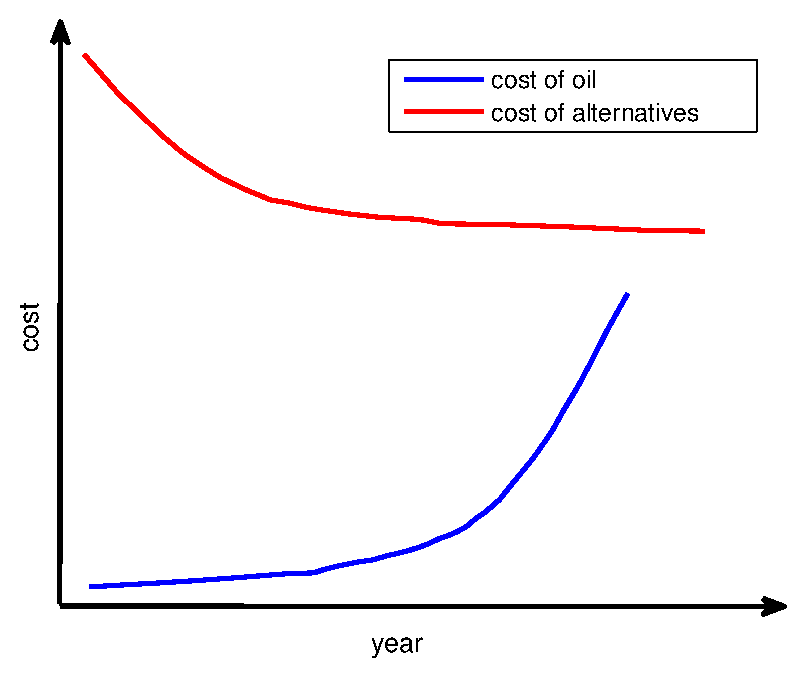
\includegraphics[width=0.6\textwidth]{fig08.eps}
\caption{The Trend of Cost for Oil and Its Alternative to Produce
unit of energy}
\end{figure}

From the trend above we get the conclusion that with the rising of
the cost for unit oil, the consumption of it will become less and
less, but its unit alternative will have low cost, and then the
demand of them will according increase, until the day when oil is
completely replaced by them. Now, the question we are faced with
is at what a speed should oil be replaced.


\subsection{Modeling}

From the above model for optimal oil distribution between
countries, we have obtained the conclusion that the growth of
consumption in future years will increase slowly. Hence, what our
research is interested in is the time when oil demand begins to
decline, i.e. the transition time of oil and its alternative.

Let GDP value to be $G$, $x$ to be the consumption of oil, $y$ to
be the consumption of the alternative, and $t$ to be time. We can
see that $G$ is a function dependent on $x$ and $y$, so

\begin{equation}
G=G(x,y)
\end{equation}


From (17), we have:

\begin{equation}
\frac{d{G}}{d{t}}=\frac{\partial{G}}{\partial{x}}\times
\frac{d{x}}{d{t}}+\frac{\partial{G}}{\partial{y}}\times
\frac{d{y}}{d{t}}
\end{equation}

During the anaphase of oil consumption, we want to keep it at a
low level in order to assure a smooth transition. We think that an
exponential decline will seem to be reasonable, so we let:

\begin{equation}
x(t)=x(t_{0})\times e^{b\times (t-t_{0})}(t>t_{0},b<0)
\end{equation}

then

\begin{equation}
\frac{d{x}}{d{t}}=x(t_{0})\times b\times e^{b\times (t-t_{0})}
\end{equation}

\begin{vardesc}{Where}$b$ :the decline rate of oil consumption;

$x(t)$ :oil consumption at year $t$.

$t_{0}$:the time when oil demand begins to decline.
\end{vardesc}

Substitute (20) into (18),and then we get:

\begin{equation}
\frac{d{y}}{d{t}}=\frac{\frac{d{G}}{d{t}}+x(t_{0})\times b\times
e^{b\times (t-t_{0})}\times \frac{\partial{G}}{\partial{x}}
}{\frac{\partial{G}}{\partial{y}}}
\end{equation}


$\frac{d{y}}{d{t}}$ denotes replacement rate,
$\frac{\partial{G}}{\partial{x}}$ means the contribution rate of
oil to GDP,and $\frac{\partial{G}}{\partial{y}}$ means the
contribution rate of the alternative to GDP. After we have known
the value of $b$, $t_{0}$, $\frac{d{G}}{d{t}}$,
$\frac{\partial{G}}{\partial{x}}$ and
$\frac{\partial{G}}{\partial{y}}$, the replacement ratio of the
alternative --- $\frac{d{y}}{d{t}}$, can be calculated, and with
the information of $\frac{d{y}}{d{t}}$, we can work out the
consumption of the alternative which will guarantee a stable
economy. This consumption works as a guidance when we exploit the
alternative. Next, we choose the year 2010 as $t_{0}$ and then
simulate to study the consumption of oil and the alternative. The
result is shown in the following figure:

\begin{figure}[!htb] \centering
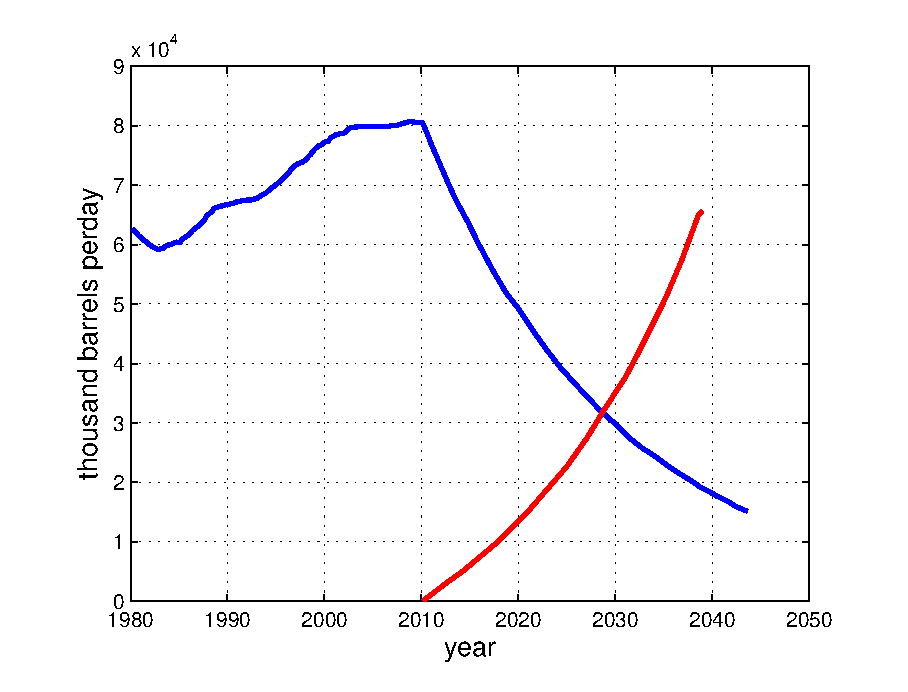
\includegraphics[width=0.7\textwidth]{fig09.eps}
\caption{The Curves of the Daily Consumption of Oil and Its
Alternative During the Transition Time}
\end{figure}

Thus, we can determine the quantity of the alternative to be
exploited which will assure the sustainable development of the
economy.

\subsection{Improvements of the Model}
As for the case where more than one alternative is available, we
can also solve the problem using the method above. But the degree
of exploitation difficulty is involved. To this end, we've
searched for some information, and have drafted the following
report. In this report, we've specifically introduced some
alternatives for oil, and hope this will pave the way for future
work.


\begin{center}
\textbf{Alternative Energy and Potential Oil Substitutes}
\end{center}

Oil, a kind of nonrenewable resource, will be used up in the near
future.

As it is pointed by C.J. Campbell ----- " The coming oil crisis
will be just that because the transition will not be easy, but I
sometimes think that the world needs a change in direction in any
case. From the ashes of the oil crisis may arise a better and more
sustainable planet. It must at least become more sustainable as
mankind lives out his allotted life span in the fossil record.
Whether or not it is better depends on how well we manage the
transition."

Transition to an entirely renewable sustainable energy resource
economy with resulting changes in lifestyles is inevitable. Will
it be done with intelligence and foresight or will it be done by
harsh natural forces? This is one of the main challenges, which
lie before us.

The crisis is imminent. Those who anticipate can do well from the
economic and political discontinuity; those who react can survive;
but those who continue to live in the past will suffer. And we
don't have long to prepare.

In this report, alternative energy and related technologies will
be talked about.

\textbf{Alternative energy:}


Alternative energy refers to energy sources, which are not based
on the burning of fossil fuels or the splitting of atoms. The
renewed interest in this field of study comes from the undesirable
effects of pollution (as witnessed today) both from burning fossil
fuels and from nuclear waste byproducts. Fortunately there are
many means of harnessing energy, which have less damaging impacts
on our environment. Here are some possible alternatives:

\textbf{Solar energy:}


 Solar energy is one the most resourceful
sources of energy for the future. One of the reasons for this is
that the total energy we receive each year from the sun is around
35,000 times the total energy used by man. However, about 1/3 of
this energy is either absorbed by the outer atmosphere or
reflected back into space (a process called albedo).

Using solar energy provide a ticket for the environmental lobby.
Solar energy is presently being used on a smaller scale in
furnaces for homes and to heat up swimming pools. On a larger
scale use, solar energy could be used to run cars, power plants,
and space ships. But the restrictions are: A huge number of solar
panels, which are not cheap, and of course, less sun means less
power, so it's not fit in countries where sunshine is not a
constant.

\textbf{Wind power:}


Wind power is another alternative energy source that could be used
without producing by-products that are harmful to nature. And
human have a long history of using wind power in the form of
windmill. Like solar power, harnessing the wind is highly
dependent upon weather and location. The average wind velocity of
Earth is around 9 m/sec. And the power that could be produced when
a windmill is facing the wind of 10 mi/hr. is around 50 watts.

\textbf{Geothermal energy:}


Geothermal energy is an alternative energy source, although it is
not resourceful enough to replace more than a minor amount of the
future's energy needs. Geothermal energy is obtained from the
internal heat of the planet and can be used to generate steam to
run a steam turbine. This in turn generates electricity, which is
a very useful form of energy.

Because of the costs required in upkeep and the shortage of
potential sites, geothermal energy systems are more inefficient
than other alternative energy sources.


\textbf{Hydroelectricity:}


Hydroelectricity comes from the damming of rivers and utilizing
the potential energy stored in the water. As the water stored
behind a dam is released at high pressure, its kinetic energy is
transferred onto turbine blades and used to generate electricity.
This system has enormous costs up front, but has relatively low
maintenance costs and provides power quite cheaply. In the United
States approximately 180,000 MW of hydroelectric power potential
is available, and about a third of that is currently being
harnessed.

\textbf{Tide:}


Similar to the more conventional hydroelectric dams, the tidal
process utilizes the natural motion of the tides to fill
reservoirs, which are then slowly discharged through
electricity-producing turbines. The former USSR produced 300 MW in
its Lumkara plant using this method.

\textbf{Oil substitutes:}

Biodiesel is made entirely from vegetable oil, it does not contain
any sulfur, aromatic hydrocarbons, metals or crude oil residues.
The absence of sulfur means a reduction in the formation of acid
rain by sulfate emissions which generate sulfuric acid in our
atmosphere. The reduced sulfur in the blend will also decrease the
levels of corrosive sulfuric acid accumulating in the engine
crankcase oil over time.

The lack of toxic and carcinogenic aromatics (benzene, toluene and
xylene) in Biodiesel means the fuel mixture combustion gases will
have reduced impact on human health and the environment. The high
cetane rating of Biodiesel (ranges from 49 to 62) is another
measure of the additive's ability to improve combustion
efficiency. Unlike other "clean fuels" such as compressed natural
gas (CNG), Biodiesel and other biofuels are produced from
renewable agricultural crops that assimilate carbon dioxide from
the atmosphere to become plants and vegetable oil. The carbon
dioxide released this year from burning vegetable oil Biodiesels,
in effect, will be recaptured next year by crops growing in fields
to produce more vegetable oil starting material. But unfortunately
it haven't been putted into wide use.


\textbf{Gas hydrate} is an ice-like crystalline solid, its
building blocks consist of a gas molecule surrounded by a cage of
water molecules. Thus, it is similar to ice, except that the
crystalline structure is stabilized by the guest gas molecule
within the cage of water molecules. Many gases have molecular
sizes suitable to form hydrate, including such naturally occurring
gases as carbon dioxide, hydrogen sulfide, and several
low-carbon-number hydrocarbons, but most marine gas hydrates that
have been analyzed are methane hydrates. They occur in the pore
spaces of sediments, and may form cements, nodes or layers.
\textbf{Gas Hydrate} is found in sub-oceanic sediments in the
polar regions (shallow water) and in continental slope sediments
(deep water), where pressure and temperature conditions combine to
make it stable.


\textbf{Gas hydrate is an important topic for study for three
reasons:}

It contains a great volume of methane, which indicates a potential
as a future energy resource

It may function as a source or sink for atmospheric methane, which
may influence global climate

It can affect sediment strength, which can initiate landslides on
the slope and rise

Other things may be used as a substitute of oil. For example, some
countries confronted with the oil crisis use \textbf{ethanol} as a
substitute of oil. Although these substitutes may provide a
possible outlet to the oil crisis, whether they can solve the
energy problem is really unknown.


\textbf{Conclusion:}


Considering the concurrent problems of population size and
stabilization, the adjustment of economies and lifestyles, the
challenge of conversion to alternative energy resources is clearly
exigent and formidable. A realistic appraisal of the future
encourages people to properly prepare for the coming events. Delay
in dealing with the issues will surely result in unpleasant
surprises. Let us get on with the task of moving orderly into the
post-petroleum paradigm.

\newpage

\begin{thebibliography}{1}
\bibitem{1} Data of world population \\http://www.cpirc.org
\bibitem{2} Chris Nelder, Oil Crises Delay�CA World Price Forecast,$2004$,\\http://www.betterworld.com
\bibitem{3} Data of oil demand, supply, reserves, and emission of $\textrm{CO}_{2}$ \\http://www.eia.doe.gov
\bibitem{4} C.J Campbell, The Coming Oil Crisis, Published by MULTI-SCIENCE PUBLISHING CO.LTD.
1997
\bibitem{5} Raymond Vernon, The Oil Crisis, Published by George J. McLeod Limited, Toronto
\bibitem{6} Atmospheric $\textrm{CO}_{2}$ concentrations (ppmv),\\
http://serc.carleton.edu/files/introgeo/interactive/examples/mlco2.doc
\bibitem{7} http://www.cc.utah.edu
\bibitem{8} Alternative resources \\http://curtrosengren.typepad.com
\bibitem{9} Alternative resources \\http://www.hubbertpeak.com
\bibitem{10} Alternative resources \\http://www.cytoculture.com
\bibitem{11} Alternative resources \\http://www.epa.gov/
\bibitem{12} Gas Hydrate web sites, \\http://woodshole.er.usgs.gov/project-pages/hydrates/external.html

\end{thebibliography}

\end{document}
